\section{History based security specifications}
Our approach must specifically be able to encode and evaluate \emph{dynamically} changing privacy constraints on a certain subset of relevant information. Additionally, these pieces of information are also dynamic and constantly changing while our system under test is actively operating. This poses several challenges in regards to how we can specify these constraints over the whole body of information beforehand. 
Instead we have decided to utilise a \emph{history} based encoding scheme, that takes the sequential nature of privacy changes over several time steps into account.
\subsection{What constitutes a history}
We rely on a central data structure, a sequential \emph{history} of abstract events, that each encode a high level operation depending on the system under test.
Formally, we can thus define any history \(h\) as
\[
    h_n = \{ev_1,ev_2,\dots, ev_n\},
\]
where \(n\) denotes the size of the given history and any \(ev_i\) represents the \(i\)-th operation or \emph{event} in the history.
Given that the history itself is in no way responsible for the way in which it is interpreted, we impose no requirements on the internal structure of the event type.
\subsection{Generating histories for HAGRID}
Given our general definition of a history, we can now look at the content of histories that we use to test our model of HAGRID. 
As described in chapter \ref{sec:hagrid_structure}, we want to be able to describe the process of verifying a given subset of valid identities belonging to a PGP key and similarly revoking these identities in a similar fashion. Note that these two operations, \emph{verifying} and \emph{revoking} identities are the central operations, that drive the dynamic declassification and reclassification of private data in our server.
We therefore define 3 abstract types of events, that can be included in a history: 
\begin{enumerate}
    \item \emph{Upload(k)} -- Given some key \(k\), this event describes the action of adding a fresh PGP key to the internal state of our server.
    \item \emph{Verify(ids,fingerprint)} -- Given a set of identities, this event describes the action of \emph{declassifying} these formerly private identities, given that they belong to the key identified by the corresponding \emph{fingerprint}
    \item \emph{Revoke(ids, fingerprint)} -- Given a set of identities, this event describes the action of \emph{reclassifying} these formerly public identities, given that they belong to the key identified by the corresponding \emph{fingerprint}
\end{enumerate}

\subsection{How to evaluate histories}
Given a history of some arbitrary size, we now require a method of inspecting the sequence of events and compute the \emph{effect} that each event in the history has on the privacy state space of our server. 
Specifically, our goal is to run a symbolic execution of a history, which ultimately computes the totality of valid visibility associations between keys and their identities. Note, that this symbolic history execution doesn't have to match the actual execution process, because we can omit the server model as our middle man and compute the privacy state for all keys directly.

\paragraph{A formal description of history evaluation}
\label{sec:history_def}
The first step of evaluating a history requires us to divide the data contained in the history into three distinct maps \(U,C\) and \(R\), where \(U\) holds an entry for every uploaded key mapping the fingerprint to the key itself. \(C\) then maps each identity which remains \emph{confirmed} at the end of the history to the fingerprint of its parent key. \(R\) on the other hand, maps all identities which remain revoked to its parent key.

Formally, these three sets can now be defined as: 

\begin{equation}
    \begin{aligned}
        U =& \{(k.fingerprint,k)  \mid k \in H(\text{Upload}) \} \\
        C =& \{(i, fingerprint_i) \mid i \in H(\text{Verify}) \wedge \phi(i, H_n) \} \\
        R =& \{(i, fingerprint_i) \mid i \in H(\text{Revoke}) \wedge \neg \phi(i,H_n)\}
    \end{aligned}
\end{equation}
   where \(\phi\) is defined as 
\begin{equation}
    \phi(i,H_n) = \exists e_t\in H(\text{Verify}) ( i \in e.ids \wedge (\forall e_k \in H(\text{Revoke}) k < i  ))
\end{equation}
 
As an end result, we want to obtain a map, that associates the fingerprint of every uploaded key to a set of \mintinline{scala}{(Identity,Status)} tuples. In this case, \mintinline{scala}{Status} indicates the visibility of the associated identity, which may take either of the following three values: 
\begin{itemize}
    \item \emph{Public} -- The identity has been declassified and can be made publicly available.
    \item \emph{Private} -- The identity remains classified and must therefore not be leaked by the server.
    \item \emph{Revoked} -- The identity has been reclassified after having been confirmed at some prior point in the history.
\end{itemize}

\textbf{TODO: formalize withUploaded, etc. }

\paragraph{History evaluation against a server model}
Determining which associations between identities and keys are valid based on a history alone is only the first step of actually \emph{testing} HAGRID. To complete our history based approach, we require a way of comparing the results of the symbolic history execution to the actual server state. Only then can we determine, whether the model adheres to our chosen privacy constraints.
The solution to this requirement consists of two parts in total. As a first step, we need to \emph{execute} the history on a given server backend. In a second step, we can then collect all available data from the server and compare the results to our previously computed visibilities. 
\\ \\
In order to visualize the execution of a history, we can look at the following example: 
\begin{figure}[H]
    \label{fig:history}
    \centering
    \makebox[\textwidth][c]{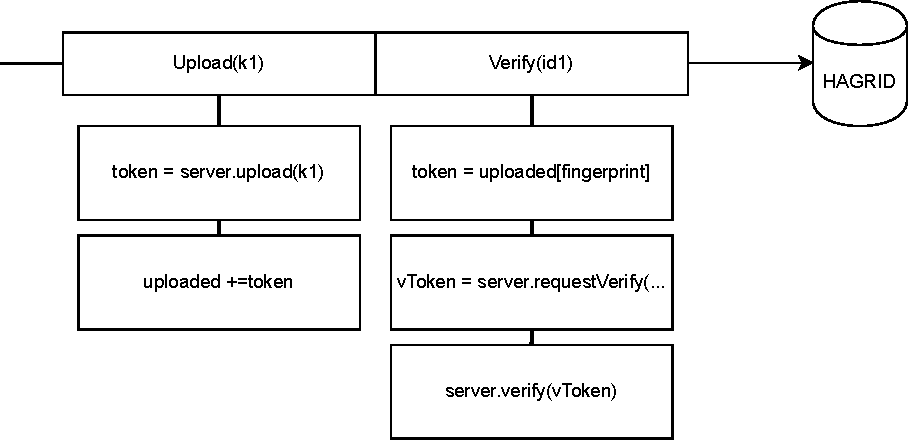
\includegraphics[width=1.1\textwidth]{images/history_small.pdf}}%
    \caption{An example of a history execution}
\end{figure}

\todo{More examples here!}

Notice, how \mintinline{Scala}{Verify} abstracts over the two separate steps of \emph{requesting} a verification and the subsequent actual verification step.
\textbf{TODO}
The algorithm for testing HAGRID can then be summarized as: 
\begin{enumerate}
    \item Using all keys contained in the given history, send a key-request to HAGRID for every key $k$
    \item Collect all returned identities in a map that associates each fingerprint with the corresponding set of identities: $ \text{fingerprint} \rightarrow \text{identities}$
    \item\label{sec:comp_hagrid} For all keys contained in either the given history, or the server response: Compare the symbolic execution result $\{(\text{Identity},\text{Status})\}$ with the matching server response $\{\text{Identity}\}$.
\end{enumerate}

\paragraph{Determining invalid associations}
Focusing on the last, third step, all that is left now is to compute all differing entries. Given that the format of both structures is very similar, this process is very straight forward.

During this evaluation step, we choose between two different result types: \mintinline{Scala}{Ok} or \mintinline{Scala}{Mismatch}.
These results are determined by comparing the \mintinline{Scala}{State} of some Identity with the corresponding Identity returned by HAGRID. For this purpose we can define the following function \(d(s_i,h_i)\)): 
\[
    d(s,h) = \begin{cases}
        \text{Ok} & \text{if } s = \epsilon \wedge h = \epsilon \\
        \text{Ok} & \text{if } s = \epsilon \wedge h_2 = \text{Private} \\
        \text{Ok} & \text{if } s = \epsilon \wedge h_2 = \text{Revoked} \\
        \text{Ok} & \text{if } s \neq \epsilon \wedge h_2 = \text{Public} \\

        \text{Mismatch} & \text{if } s \neq \epsilon \wedge h = \epsilon \\
        \text{Mismatch} & \text{if } s = \epsilon \wedge h_2 = \text{Public} \\
        \text{Mismatch} & \text{if } s \neq \epsilon \wedge h_2 = \text{Private} \\
        \text{Mismatch} & \text{if } s \neq \epsilon \wedge h_2 = \text{Revoked} 
    \end{cases}    
\]

where \(\epsilon\) denotes the absence of a value.

